% =====================================================================
%  Kollisionskaskaden -- Kurze Physik-Praesentation
%  Paul Kamm, TH Luebeck, betreut von Dr. Maurice Maurer
%
%  Bau:  pdflatex physik_praesentation.tex   (2x fuer Referenzen)
%
%  Aufbau: 7 Folien, 2 Videos.
%    1 Das Modell                    5 Clusterdefinition angepasst
%    2 Video: Geschwindigkeitspeak   6 Neues Ergebnis
%    3 Video: Defektcluster          7 Plan fuer die Bachelorarbeit
%    4 Projektergebnis / ueberprueft
%  Danach Reservefolien (Anhang, nicht Teil des Vortrags).
%
%  Videos: die MP4s liegen separat in videos/. Jede Video-Folie zeigt ein
%  Standbild aus stills/ und bindet den Film auf zwei Wegen ein:
%
%    1. \movie (Paket multimedia) legt eine Screen-Annotation ueber das
%       Standbild. pdfpc und Okular spielen den Film damit INLINE ab.
%    2. Die Zeile darunter ist eine Launch-Action (run:), die den
%       Systemplayer oeffnet -- das koennen Acrobat und einige andere.
%
%  Firefox/pdf.js kann WEDER das eine NOCH das andere: es ignoriert
%  Launch-Actions und Screen-Annotationen stillschweigend. Zum Vortragen
%  daher pdfpc (empfohlen) oder Okular verwenden:
%
%      pdfpc physik_praesentation.pdf
%
%  Notfalls videos/index.html im Browser oeffnen und dort abspielen.
% =====================================================================
\documentclass[aspectratio=169,11pt]{beamer}

\usetheme{metropolis}
\usepackage[ngerman]{babel}
\usepackage[utf8]{inputenc}
\usepackage[T1]{fontenc}
\usepackage{amsmath,amssymb}
\usepackage{graphicx}
\usepackage{booktabs}
\usepackage{multimedia}
\usepackage{tikz}

% --- Farben: tiefes Blau + warmes Orange (Kaskaden-Motiv) ------------
\definecolor{tiefblau}{RGB}{20,28,60}
\definecolor{glut}{RGB}{235,110,40}
\setbeamercolor{frametitle}{bg=tiefblau, fg=white}
\setbeamercolor{progress bar}{fg=glut}
\setbeamercolor{alerted text}{fg=glut}
\metroset{block=fill, numbering=fraction, progressbar=frametitle}

\graphicspath{{stills/}{figures/}{../results/images/}{./}}

% Bequemes Makro fuer eine Video-Folie: #1 Titel, #2 Standbild, #3 mp4, #4 Bildunterschrift
% Das Standbild ist die Abspielflaeche (inline in pdfpc/Okular), die Zeile
% darunter oeffnet den Systemplayer.
\newcommand{\videofolie}[4]{%
  \begin{frame}{#1}
    \centering
    \movie[showcontrols, borderwidth=0pt]%
      {\includegraphics[height=0.72\textheight]{#2}}{videos/#3}\\[0.3em]
    {\footnotesize #4 \quad\alert{$\blacktriangleright$
      \href{run:videos/#3}{extern öffnen}}}
  \end{frame}}

\title{Kollisionskaskaden}
\subtitle{Strahlenschaden in einem 2D-Modellkristall}
\author{Paul Kamm}
\institute{TH Lübeck \, ·\, betreut von Dr.\ Maurice Maurer}
\date{}

\begin{document}

\maketitle


% ===================================================================== 1
% \begin{frame}{Warum ein Minimalmodell?}
%   \begin{columns}[T]
%     \begin{column}{0.5\textwidth}
%       {\small \textbf{Das Problem}
%       \begin{itemize}
%         \item Die erste Wand eines Fusionsreaktors ist aus \alert{Wolfram}
%           und steht im Fluss von 14-MeV-Neutronen.
%         \item Ein Neutron stößt ein Gitteratom an -- das \alert{PKA}. Es
%           löst in Pikosekunden eine \alert{Kollisionskaskade} aus.
%         \item Zurück bleiben Defektcluster: Versprödung, begrenzte
%           Lebensdauer der Wand.
%       \end{itemize}}
%     \end{column}
%     \begin{column}{0.5\textwidth}
%       {\small \textbf{Warum das Statistik verlangt}
%       \begin{itemize}
%         \item Interessant ist nicht die einzelne Kaskade, sondern die
%           \alert{Verteilung} der Clustergrößen.
%         \item Eine Verteilung braucht Hunderte bis Tausende Kaskaden --
%           ein \alert{Ensemble}.
%         \item Volle Molekulardynamik: Millionen Atome pro Kaskade. Für
%           Ensembles zu teuer.
%       \end{itemize}}
%     \end{column}
%   \end{columns}
%   \begin{alertblock}{Der Ansatz}
%     {\small Nur \textbf{Massen und brechbare Federn}, zwei Dimensionen --
%     eine Kaskade in Sekunden statt Stunden.
%     \textbf{Kernfrage: Wie viel Statistik überlebt in Massen und Federn?}}
%   \end{alertblock}
% \end{frame}

% ===================================================================== 2
\begin{frame}{Das Modell}
  \leavevmode
  {\footnotesize Atome auf einem \alert{Dreiecksgitter}, jedes mit sechs
  Nachbarn. Jede Bindung ist eine \alert{Feder}, die bei 15\,\% Dehnung reißt
  und gerissen bleibt. Zu nahe Atome \alert{stoßen sich stark ab}. Das PKA ist
  ein Atom mit hoher Startgeschwindigkeit.}
  \vspace{0.3em}
  \begin{columns}[T]
    \begin{column}{0.55\textwidth}
      \centering
      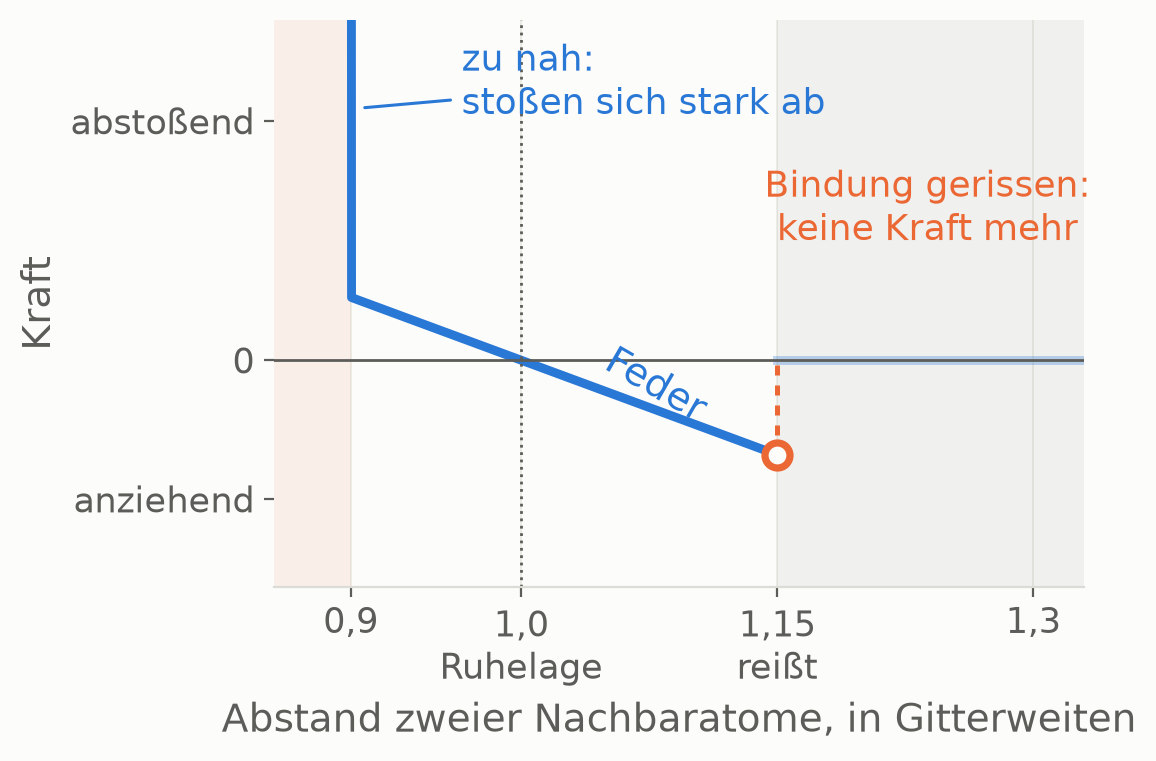
\includegraphics[height=0.58\textheight]{P2_kraft.png}\\[0.2em]
      {\scriptsize Die Kraft zwischen zwei Nachbarn.}
    \end{column}
    \begin{column}{0.43\textwidth}
      \centering
      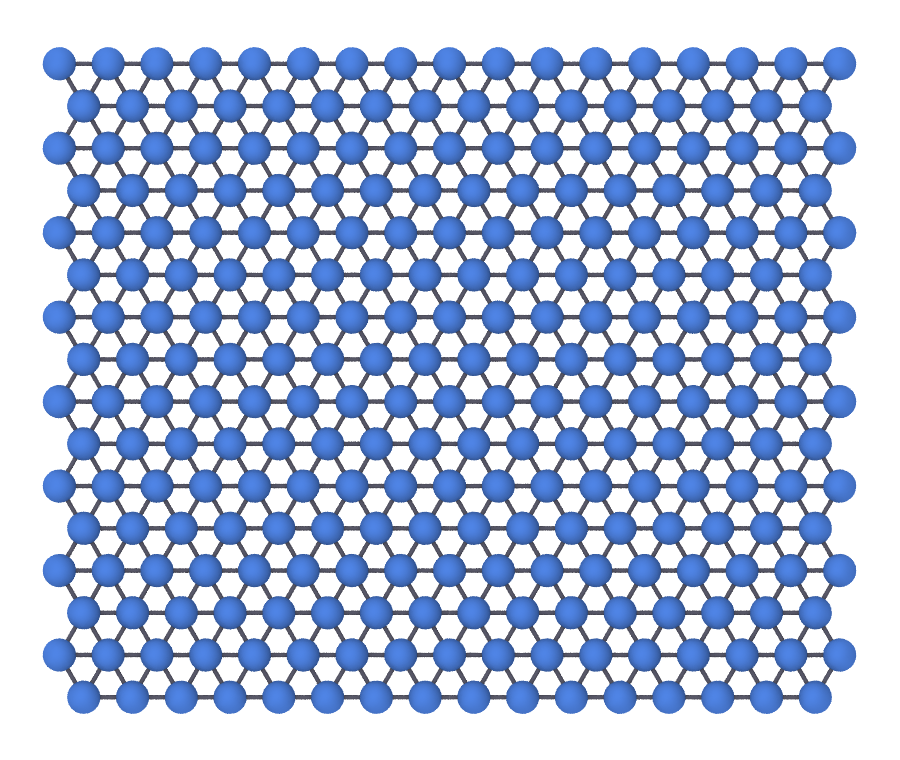
\includegraphics[height=0.58\textheight]{modell_ruhelage.png}\\[0.2em]
      {\scriptsize Das Gitter in Ruhe.}
    \end{column}
  \end{columns}
\end{frame}

% ===================================================================== 3
\videofolie{Geschwindigkeitspeak}{still_1.png}{cascade_1_geschwindigkeit.mp4}
  {Farbe = Geschwindigkeit. Die Einschlagsenergie wird zu einer heißen,
   ungeordneten Zone bewegter Atome, die expandiert und wieder abkühlt.}

% ===================================================================== 4
\videofolie{Defektcluster}{still_3.png}{cascade_3_cluster.mp4}
  {Farbig sind die Atome, die mehr als eine Gitterweite von ihrem Platz weg
   sind. \alert{Jede Farbe ist ein eigener Cluster}, grau ist das ungestörte
   Gitter.}

% ===================================================================== 5
\begin{frame}{Projektergebnis}
  \begin{columns}[T]
    \begin{column}{0.54\textwidth}
      \centering
      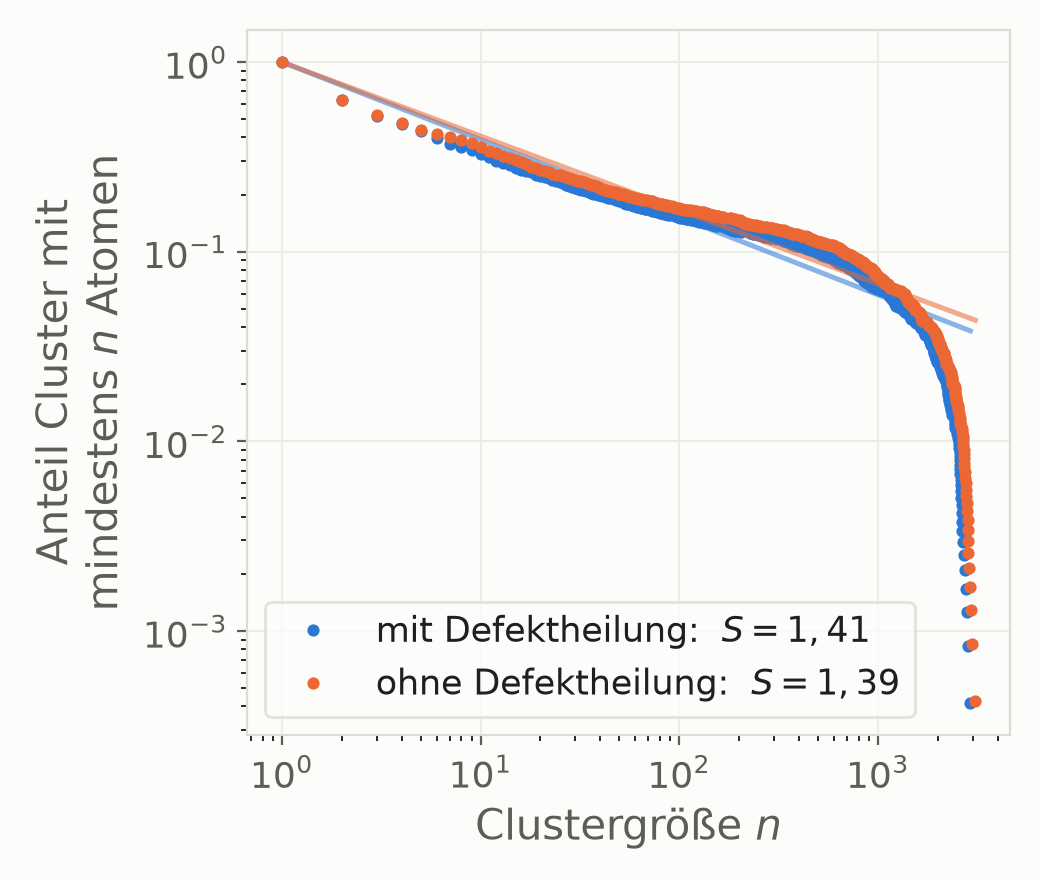
\includegraphics[width=\linewidth]{P5_ccdf_gepoolt.png}
    \end{column}
    \begin{column}{0.44\textwidth}
      {\footnotesize
      Aus 1000 Kaskaden, alle Cluster zusammengezählt, kam ein
      \alert{Potenzgesetz} heraus:
      \[ \text{Häufigkeit} \;\propto\; n^{-S},\qquad S\approx1{,}4. \]
      \vspace{-0.6em}
      \begin{itemize}
        \item Es gibt keine typische Clustergröße: kleine Cluster sind häufig,
          große selten, und das im selben Verhältnis über alle Größen hinweg.
        \item Logarithmisch aufgetragen liegen die Punkte deshalb auf einer
          \alert{Geraden}.
        \item $S$ ist die Steilheit dieser Geraden: je größer $S$, desto
          seltener die großen Cluster.
      \end{itemize}}
    \end{column}
  \end{columns}
\end{frame}

% ===================================================================== 5b
\begin{frame}{Projekt überprüft}
  \leavevmode
  {\footnotesize \textbf{Anpassungsgüte} (Goodness of Fit): Passt das
  Potenzgesetz überhaupt zu den Daten? \alert{Nein.}\\[0.5em]
  \textbf{Vergleich mit anderen Verteilungen} (Likelihood-Ratio-Test): Welche
  Kurvenform beschreibt die Daten besser?}\\[0.4em]
  {\scriptsize
  \begin{tabular}{@{}lll@{}}
    \toprule
    Verteilung & Form im Bild & Ergebnis\\
    \midrule
    Exponentialverteilung & fällt viel schneller ab & Potenzgesetz ist besser\\
    Lognormalverteilung & leicht gebogen statt gerade & \alert{beschreibt es besser}\\
    Potenzgesetz mit Cutoff & Gerade, die oben abknickt & \alert{beschreibt es besser}\\
    \bottomrule
  \end{tabular}}
  \vspace{0.7em}\hrule\vspace{0.5em}
  {\footnotesize \alert{\textbf{Begründung:}} Die Einschlagsenergie war in
  jedem Lauf zufällig, jeder Zehnerbereich gleich oft. Weil die Clustergröße
  fast nur von der Energie abhängt, entsteht die Gerade schon durch diese
  Auswahl -- gemessen haben wir also die Energieverteilung und nicht die
  Kaskade.\\[0.3em]
  Mit Sand et al.\ kann man das deshalb nicht vergleichen: dort werden rund
  100 Kaskaden bei \emph{einer} festen Energie gerechnet, hier 1000 Kaskaden
  mit zufällig gestreuten Energien.}
\end{frame}

% ===================================================================== 6
\begin{frame}{Clusterdefinition angepasst}
  % \leavevmode verhindert, dass beamer die folgende Klammergruppe als
  % Untertitel liest und stillschweigend verwirft.
  \leavevmode
  {\footnotesize \alert{900 Läufe bei fester Energie}: dreimal 300 mit
  $E=1300$, $1800$ und $2400$, jeweils an denselben Stellen und Winkeln.}
  \vspace{0.3em}
  \begin{columns}[T]
    \begin{column}{0.44\textwidth}
      {\footnotesize
      \textbf{Alte Definition:} verschoben ab 0,5 Gitterweiten,
      zusammengehörig unter 1,5. Damit wird die ganze Schadenszone
      \alert{ein} Klumpen, der 92\,\% aller verschobenen Atome enthält.\\[0.6em]
      \textbf{Neue Definition:} verschoben ab 1,0, zusammengehörig unter 1,0.
      Dieselben Atome, aber \alert{30 bis 70 getrennte Cluster} pro Lauf.
      Das zählen auch Sand et al.\\[0.6em]
      \emph{Abw.} im Bild ist der Abstand zwischen Messpunkten und Gerade,
      kleiner ist besser.}
    \end{column}
    \begin{column}{0.54\textwidth}
      \centering
      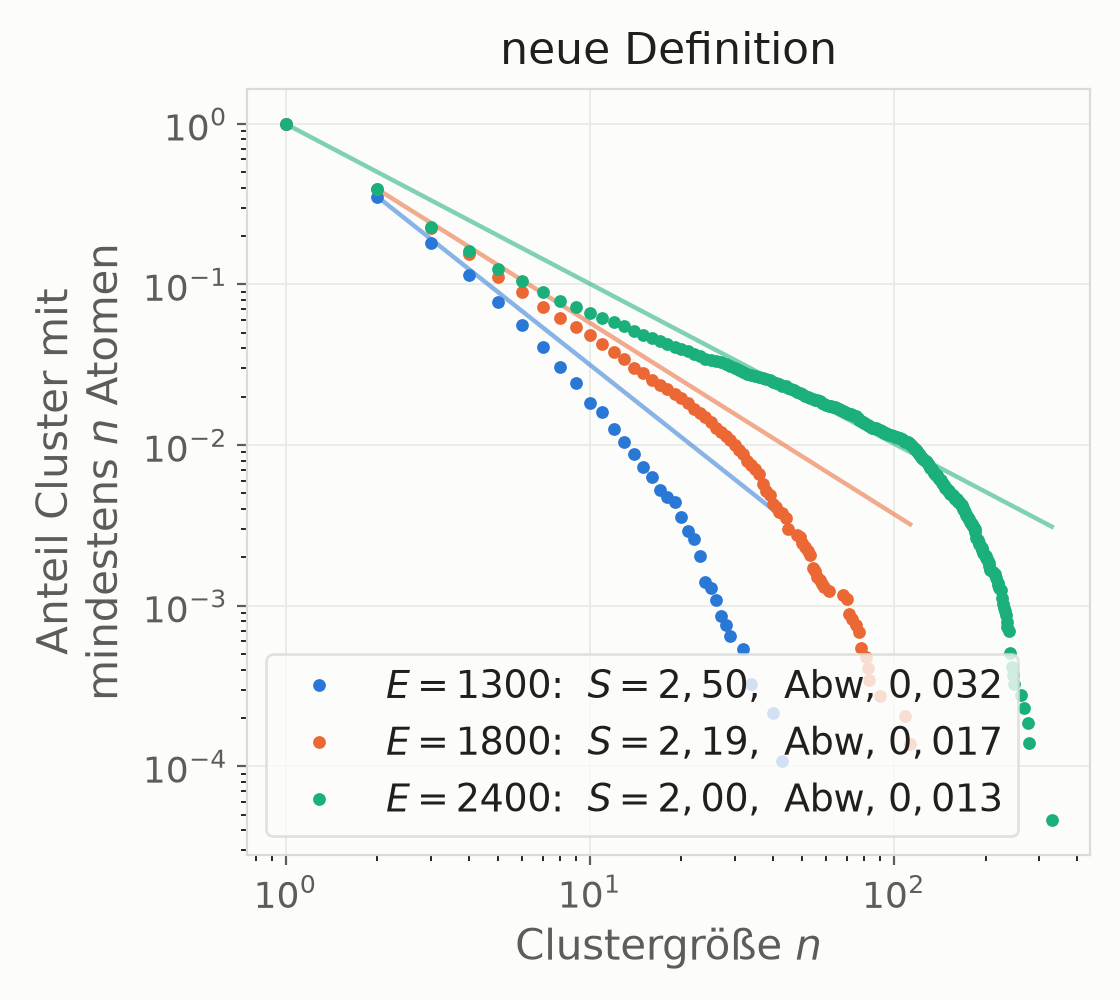
\includegraphics[width=0.80\linewidth]{P6_ccdf_fein.png}
    \end{column}
  \end{columns}
\end{frame}

% ===================================================================== 7
\begin{frame}{Neues Ergebnis}
  \begin{columns}[T]
    \begin{column}{0.56\textwidth}
      {\footnotesize
      \begin{itemize}
        \item \textbf{$S$ hängt davon ab, wie man einen Cluster definiert.}
          Sechs verschiedene Definitionen auf denselben 900 Läufen ergeben
          \alert{$S$ zwischen 1,23 und 3,30}. 
        \item \textbf{$S$ wird kleiner, je größer die Kaskade ist}
          (2,50, dann 2,19, dann 2,00), und die Gerade passt dabei immer
          besser. \alert{Wo $S$ am Ende landet, wissen wir noch nicht.}
        \item \textbf{Jetzt können wir mit Sand et al.\ (2013) vergleichen},
          denn dort wird ebenfalls bei fester Energie gerechnet. In Wolfram
          (3D) ist $S=1{,}63$, hier in 2D rund 2,0, also \alert{größer}.
          Dazu passt, dass jedes Atom in 2D weniger Nachbarn hat.
      \end{itemize}}
    \end{column}
    \begin{column}{0.42\textwidth}
      \centering
      {\scriptsize\setlength{\tabcolsep}{3.5pt}
      \begin{tabular}{@{}ccccc@{}}
        \toprule
        \multicolumn{2}{c}{Definition} & \multicolumn{3}{c@{}}{Energie}\\
        \cmidrule(r){1-2}\cmidrule(l){3-5}
        \shortstack{verschoben\\ab} & \shortstack{zusammen\\unter}
          & 1300 & 1800 & 2400\\
        \midrule
        0,5 & 1,5 & 1,40 & 1,35 & 1,23\\
        1,0 & 1,5 & 1,57 & 1,50 & 1,45\\
        0,5 & 1,0 & 1,98 & 2,10 & 2,25\\
        1,0 & 1,0 & 2,50 & 2,19 & 2,00\\
        1,5 & 1,0 & 2,78 & 2,51 & 2,28\\
        2,0 & 1,0 & 3,30 & 3,02 & 2,77\\
        \bottomrule
      \end{tabular}\\[0.4em]
      $S$ für sechs Definitionen. Die beiden\\ linken Spalten in Gitterweiten.}
    \end{column}
  \end{columns}
\end{frame}

% ===================================================================== 8
\begin{frame}{Plan für die Bachelorarbeit}
  \leavevmode
  \vspace{0.2em}
  {\footnotesize
  \begin{enumerate}
    \item \textbf{Pendelt sich $S$ auf einen Wert ein?} Bisher wird $S$ mit
      jeder Energiestufe kleiner. Das kann daran liegen, dass das Gitter mit
      $250\times250$ Atomen \alert{zu klein} ist: die größten Cluster stoßen
      an den Rand der Schadenszone. Größeres Gitter und höhere Energien
      auf einem Cluster könnten zeigen, ob $S$ gleich bleibt oder weiter fällt.
    \item \textbf{Clusterdefinition systematisch durchgehen.} $S$ für viele
      Kombinationen aus Schwelle und Abstand berechnen. Gibt es einen Bereich,
      in dem $S$ stabil bleibt? Der wäre die sinnvolle Definition.
    \item \textbf{Das Modell an Wolfram anpassen.} Federhärte, Reißdehnung und
      Abstoßung so wählen, dass die Bindungsenergie und die Energie, ab der ein
      Atom seinen Platz verlässt, zu echtem Wolfram passen.
    \item \textbf{Das Modell auf drei Dimensionen erweitern.} Dann wären die
      Literaturwerte direkt vergleichbar.
    \item \textbf{Hauptfrage:} Wenn das einfache Modell die Statistik richtig
      wiedergibt, taugt es als günstiger Vorfilter: viele
      Parameterkombinationen grob durchsuchen und die teure Molekulardynamik
      nur dort einsetzen, wo es interessant wird.
  \end{enumerate}}
\end{frame}


% =====================================================================
%  Reservefolien -- nicht Teil des Vortrags, fuer Rueckfragen.
% =====================================================================
\appendix

\begin{frame}{Reserve: Von der Tabelle zur Clustergröße}
  \centering
  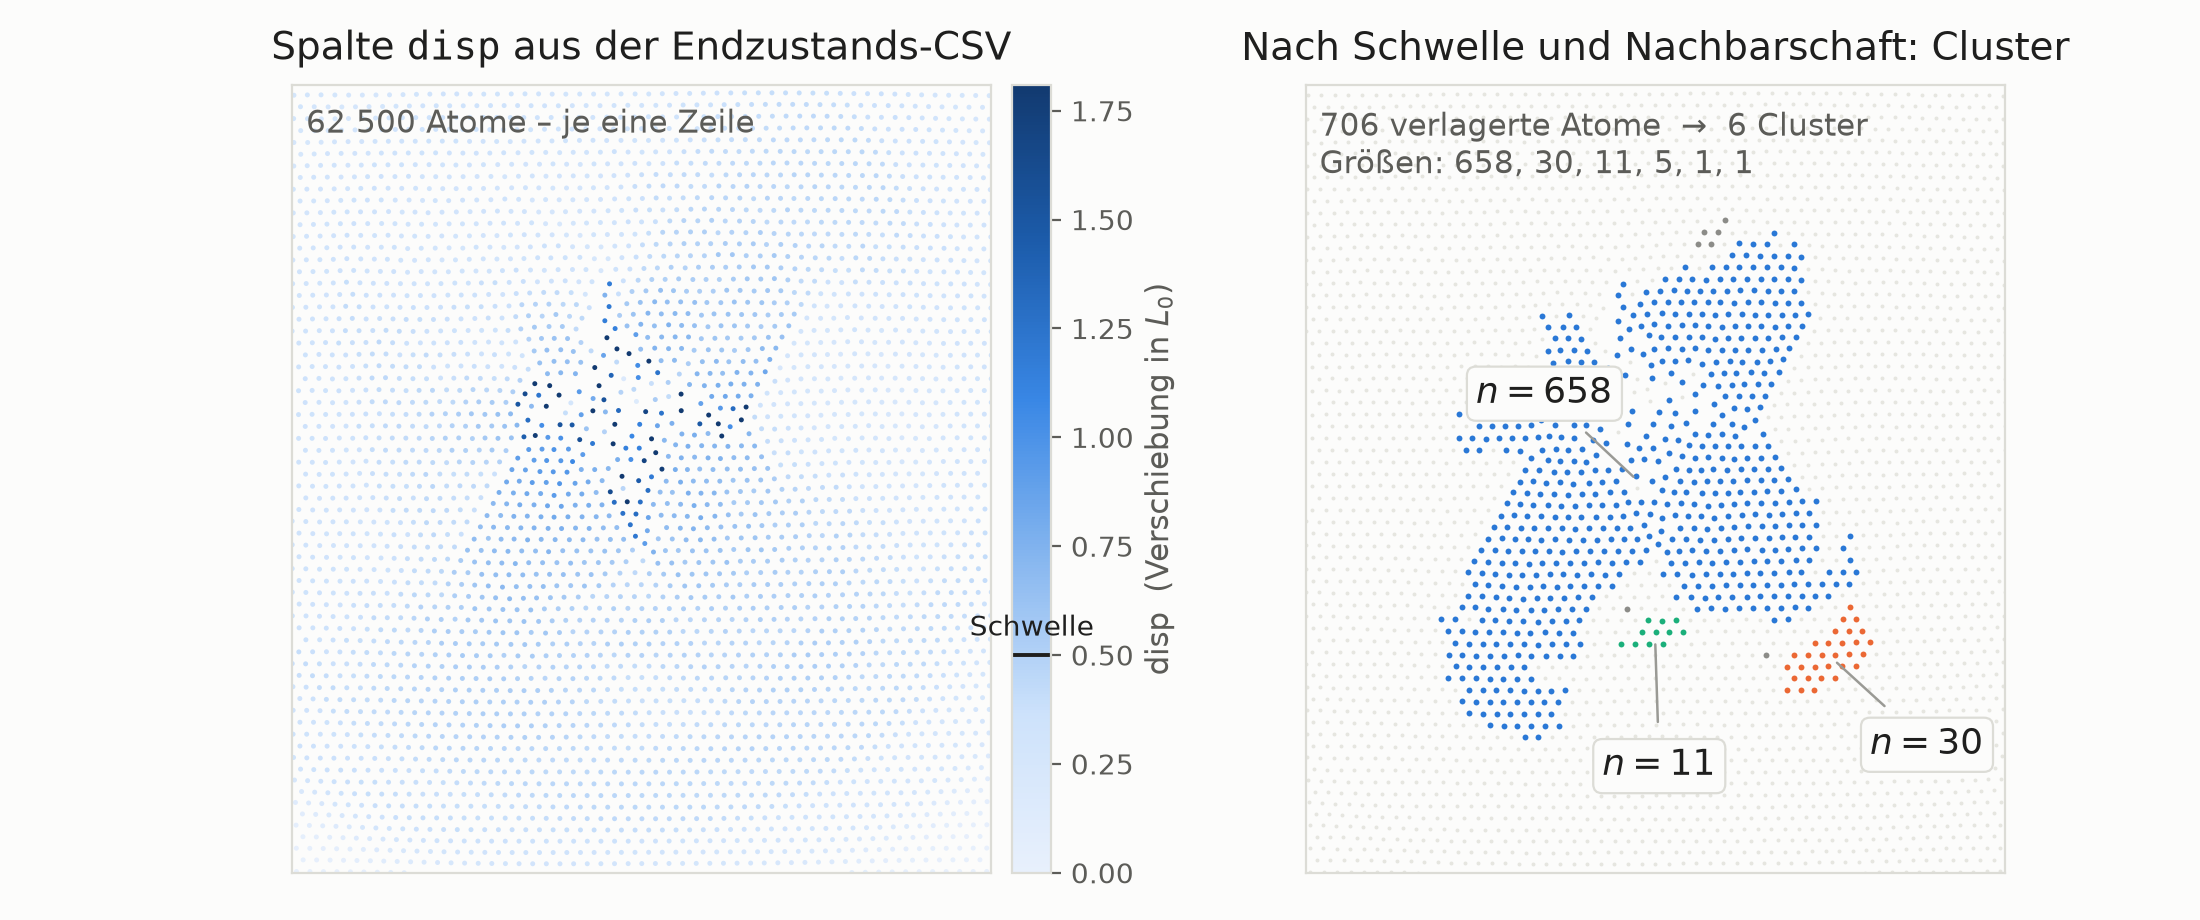
\includegraphics[width=0.88\linewidth]{P1_csv_zu_cluster.png}\\[0.4em]
  {\scriptsize
  \begin{columns}[T]
    \begin{column}{0.31\textwidth}
      \textbf{1 · Schwelle}\\
      Verlagert, wenn $\texttt{disp}>0{,}5\,L_0$, also eine halbe
      Gitterkonstante.
    \end{column}
    \begin{column}{0.31\textwidth}
      \textbf{2 · Nachbarschaft}\\
      Verlagerte Atome mit Abstand $<1{,}5\,L_0$ bilden einen Cluster;
      seine Größe $n$ ist die Zahl seiner Atome.
    \end{column}
    \begin{column}{0.31\textwidth}
      \textbf{3 · Poolen}\\
      \alert{1000 Läufe} $\to$ \alert{2391 Cluster}, $n$ von 1 bis 2920.
      Deren Häufigkeitsverteilung ist das Ergebnis.
    \end{column}
  \end{columns}}
\end{frame}

\begin{frame}{Reserve: Was ein Lauf hinterlässt}
  \begin{columns}[T]
    \begin{column}{0.53\textwidth}
      Mitgeschrieben werden drei Dinge:
      \begin{itemize}
        \item \textbf{Momentaufnahmen} während des Laufs: Ort,
          Geschwindigkeit, Verschiebung und gerissene Bindungen jedes
          Atoms. Daraus entstehen die Videos.
        \item \textbf{Energiebilanz}: kinetisch, Feder, Abstoßung,
          Bruch. Reine Kontrolle, die Summe muss erhalten bleiben.
        \item \textbf{Endzustand} nach dem Abkühlen: \alert{eine Zeile
          pro Atom}. Aus dieser Tabelle kommt die gesamte Statistik.
      \end{itemize}
    \end{column}
    \begin{column}{0.47\textwidth}
      \centering
      {\footnotesize Endzustand, $250\times250=62\,500$ Zeilen:}\\[0.4em]
      {\scriptsize
      \begin{tabular}{rrrr}
        \toprule
        \texttt{x} & \texttt{y} & \texttt{disp} & \texttt{broken}\\
        \midrule
        0.0000 & 0.0000 & 0.0000 & 4\\
        1.0000 & 0.0000 & 0.0000 & 2\\
        \multicolumn{4}{c}{$\vdots$}\\
        114.3486 & 83.5237 & 0.5040 & 0\\
        123.5459 & 98.3829 & 1.2109 & 2\\
        \bottomrule
      \end{tabular}}\\[0.7em]
      \begin{minipage}{0.95\linewidth}\raggedright\footnotesize
      \textbf{disp}: bleibende Auslenkung vom \emph{eigenen} Gitterplatz,
      in Gitterabständen $L_0$.\\[0.3em]
      \textbf{broken}: wie viele der sechs Bindungen gerissen sind.
      \end{minipage}
    \end{column}
  \end{columns}
\end{frame}

\begin{frame}{Reserve: beide Clusterdefinitionen im Vergleich}
  \centering
  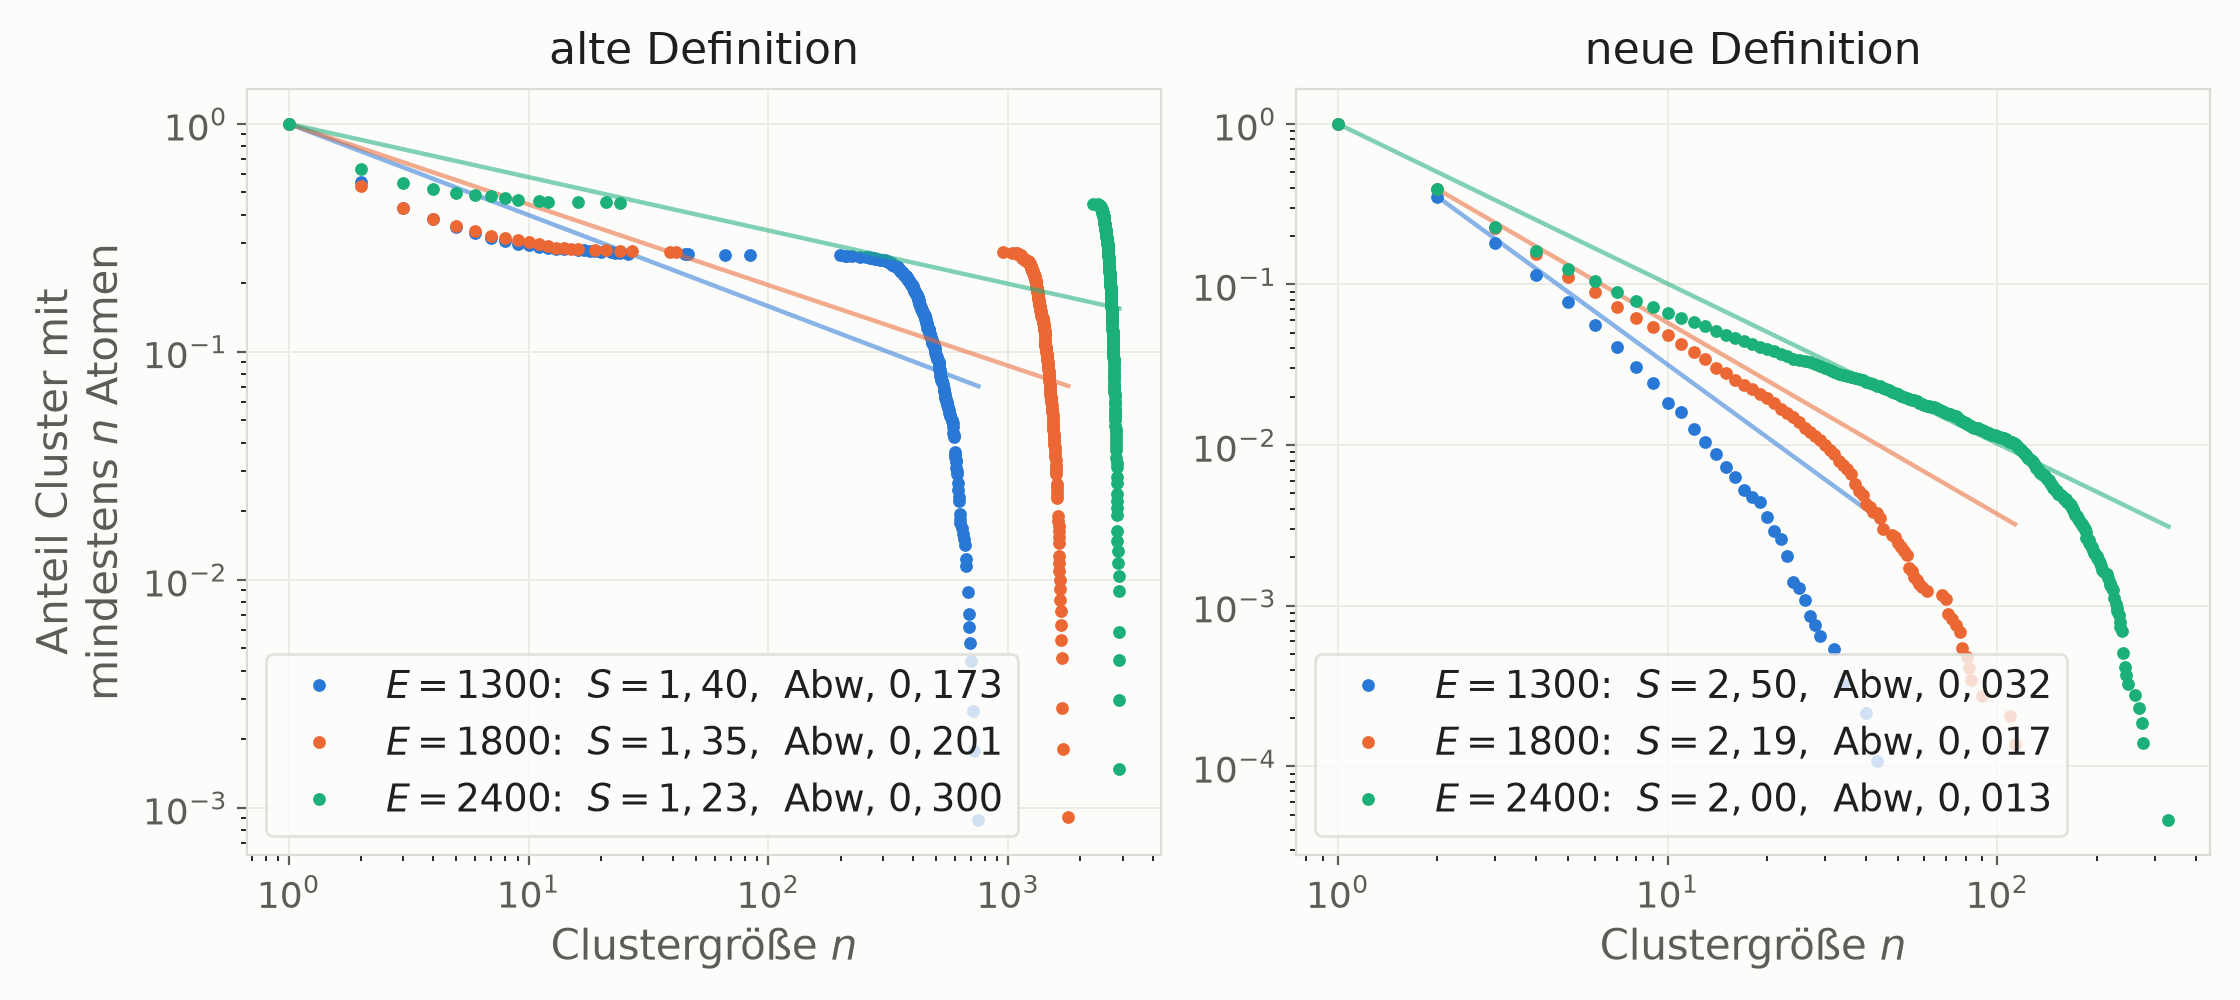
\includegraphics[width=0.98\linewidth]{P6_ccdf_beide.png}\\[0.3em]
  {\scriptsize Dieselben 900 Läufe. Links bricht die CCDF senkrecht ab --
   der eine Riesencluster. Rechts eine durchgehende Verteilung über zwei
   Größenordnungen.}
\end{frame}

\videofolie{Reserve: Die Schadensbildung}{still_2.png}{cascade_2_schaden.mp4}
  {Farbe = Zahl gerissener Bindungen. Die Defektstruktur wächst und
   \alert{friert} als bleibender Cluster ins Gitter ein.}

\videofolie{Reserve: viele Einschläge}{still_4.png}{cascade_4_mehrere_pka.mp4}
  {Fünf gleichzeitige PKAs. Überlappende Kaskaden, und ein Atom, das entlang
   einer Gitterrichtung \alert{kanalisiert} (der lange Track).}


\end{document}
